\documentclass[xcolor=svgnames,dvipsnames,table, hyperref=pdftex, mathserif, presentation]{beamer}
\usepackage{amsmath,amssymb,amsfonts,amsthm}
\usepackage{ctex}
\setCJKsansfont{KaiTi}% 文泉驿的黑体
\usepackage{graphics}
\usepackage{graphicx}
\usepackage{xcolor}
\usepackage{wasysym}
\usepackage{bbm}
\usepackage{url}
\usepackage{beamerleanprogress}
\usepackage{tikz-dependency}
\usepackage{tikz-qtree}
\usepackage{hhline}
\usepackage{fancyvrb}
\usepackage{mathrsfs}
\usepackage{alltt}
% for uml charts
\usepackage{tikz}
\usetikzlibrary{calc,arrows.meta, graphs, trees, shapes, positioning, automata,
shapes.geometric, shapes.multipart, er, patterns, decorations.markings, intersections, decorations.text}
\usepackage{tikz-uml}

\usetheme{CambridgeUS}
%\usetheme{Pittsburgh}
\usecolortheme{orchid} % seahorse  orchid rose
\setbeamertemplate{blocks}[rounded][shadow=true]
\AtBeginSection[]{%
  \begin{frame}<beamer>
    \frametitle{Outline}
      \tableofcontents[current] 
    \end{frame}
  \addtocounter{framenumber}{-1}% If you don't want them to affect the slide number
}
\AtBeginSubsection[]
{
  \begin{frame}
  \frametitle{Outline}
    \tableofcontents[currentsection,currentsubsection]
  %\tableofcontents[sectionstyle=show/hide,subsectionstyle=hide/show/hide]
  \end{frame}
  \addtocounter{framenumber}{-1}% If you don't want them to affect the slide number
}
\newcommand{\setof}[1]{\ensuremath{\left \{ #1 \right \}}}
\newcommand{\tuple}[1]{\ensuremath{\left \langle #1 \right \rangle }}
\newcommand{\red}[1]{\textcolor{red}{#1}}
\newcommand{\brown}[1]{\textcolor{brown}{#1}}
\newcommand{\green}[1]{\textcolor{green}{#1}}
\newcommand{\blue}[1]{\textcolor{blue}{#1}}
\newcommand{\cyan}[1]{\textcolor{cyan}{#1}}

%gets rid of navigation symbols
%\setbeamertemplate{navigation symbols}{}

\begin{document}

\title[Retrofitting]{Retrofitting Word Vectors to Semantic Lexicons \[NAACL2015\]}

\institute[icst@pku]{
  Carnegie Mellon University
}
\author[Han Zhe]{
  Manaal Faruqui, Jesse Dodge\\
  Sujay K. Jauhar, Chris Dyer\\
  Eduard Hovy, Noah A. Smith\\
}

\frame[t,plain]{ \titlepage } % [t,plain]

\frame{
  \frametitle{ Outline  }
  
   \begin{itemize}
      \item 论文方法概述

      \item 传统词向量生成工具
	  \begin{itemize}
	   \item Glove, Skip-Gram, Global Context, Multilingual Vectors
	  \end{itemize}

      \item 语义词典(Semantic Lexicon)
	  \begin{itemize}
	   \item PPDB, WordNet, FrameNet
	  \end{itemize}
      
      \item 实验
	  \begin{itemize}
	   \item 数据集
	      \begin{itemize}
	       \item Word Similarity: WS-353, RG-65, MEN
	       \item Syntactic Relations, Synonym Selection, Sentiment Analysis
	      \end{itemize}
	  \item 顺序模型:Retrofitting with Semantic Lexicons
	  \item 联合模型:Semantic Lexicons during Learning
	      \begin{itemize}
	      \item lazy method, periodic method
	      \end{itemize}
	  \item 实验分析
	  \end{itemize}
   \end{itemize}

}

\frame{
  \frametitle{Summary}
  论文方法概述\\
  \vspace{5mm}
  \begin{itemize}
   \item 把语义信息加入词向量;语义相关的单词词向量有更大的相似性
   \item 两类方法
      \begin{itemize}
       \item 顺序模型:先使用传统词向量生成工具,再使用语义信息修正词向量
       \item 联合模型:修正传统词向量训练时的目标函数,在其中加入语义信息
      \end{itemize}

  \end{itemize}

}


\frame{
  \begin{columns}[c]
   \column{.15\hsize}
   \column{.7\hsize}
   \begin{block}{}
    \centering \Large 传统词向量生成工具
   \end{block}

   \column{.15\hsize}
  \end{columns}

}

\frame{
  \frametitle{传统词向量生成工具tools}
  \begin{columns}[c]
      \column{0.4\hsize}
      \begin{block}{Glove}
	  \begin{itemize}
	   \item stanford:Jeffrey Pennington,   Richard Socher
	   \item 收集单词对的共线情况
	  \end{itemize}
      \end{block}

      \begin{block}{word2vec}
       Skip-Gram Vectors
      \end{block}

      \column{0.4\hsize}
      \begin{block}{Global Context Vector}
       tree-RNN + local and global (document) context features
      \end{block}
      
      \begin{block}{Multilingual Vector}
       SVD + CCA
      \end{block}
  \end{columns}

}

\frame{
  \begin{columns}[c]
   \column{.15\hsize}
   \column{.7\hsize}
   \begin{block}{}
    \centering \Large 语义词典
   \end{block}

   \column{.15\hsize}
  \end{columns}

}

\frame{
  \frametitle{Semantic Lexicon}
      \begin{block}{PPDB}
	  \begin{itemize}
	   \item 复述(paraphrase)预料集
	   \item 220 million paraphrase pairs
	   \item 6个版本:S,M,L,XL,XXL,XXXL,容量依次增大,质量依次降低
	   \item \small [VBN] ||| pruned ||| cropped ||| p(e|f)=4.33 p(f|e)=4.88 ... ||| 0-0
	  \end{itemize}
      \end{block}
  \begin{columns}[c]
      \column{0.5\hsize}
      \begin{block}{FrameNet}
	  \begin{itemize}
	   \item \tiny frame:$Cause\_change\_of\_position\_on\_a\_scale$ $\leftrightarrow{push, raise,..., growth}$
	  \end{itemize}

       
      \end{block}
      
      \column{0.4\hsize}
      \begin{block}{WordNet}
       $WN_{syn}$: 只对同义词连边
       $WN_{all}$: 同义词、上位词、下位词都连边
      \end{block}
      
  \end{columns}
   
  \vspace{2mm}
  实验时$\alpha_i=1,\beta_{ij}=degree(i)^{-1}$
}


\frame{
  \begin{columns}[c]
   \column{.15\hsize}
   \column{.7\hsize}
   \begin{block}{}
    \centering \Large 实验数据集
   \end{block}

   \column{.15\hsize}
  \end{columns}

}

\frame{
  \frametitle{Word Similarity}
  
  \begin{columns}[c]
   \column{0.5\hsize}
  \begin{block}{WS-353}
   \begin{itemize}
    \item 353个英语单词对(200个13个人标,153个16个人标)
    \item 相似度:0-10(可0.5)
   \end{itemize}
  \end{block}
   
   \column{0.45\hsize}
  \begin{block}{RG-65}
   \begin{itemize}
    \item 65对英语名词
   \end{itemize}
  \end{block}
  
  \begin{block}{MEN}
   \begin{itemize}
    \item 3000对单词(共现700次)
   \end{itemize}
  \end{block}
   
  \end{columns}

  \pause
  \vspace{2mm}
  评价结果好坏采用斯皮尔曼等级相关系数
  \vspace{1mm}
  
  \begin{columns}[c]
   \column{0.4\hsize}
   \centering 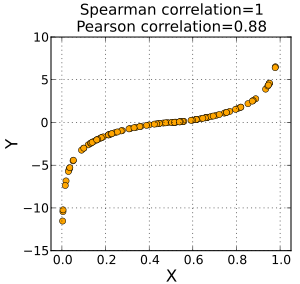
\includegraphics[width=0.7\hsize]{file/Spearman.png}
   
   \column{0.55\hsize}
   $\rho=\frac{\sum_i(x_i-\bar{x})(y_i-\bar{y})}{\sqrt{\sum_i(x_i-\bar{x})^2\sum_i(y_i-\bar{y})^2}}\in [-1,1]$
  \end{columns}


}

\frame{
  \frametitle{}
  \begin{block}{Syntactic Relation(SYN-REL)}
      \begin{itemize}
       \item Mikolov给出(word2vec)
       \item 给定a,b,c,找到最合适的d,满足:a is to b as c is to d
       \item 实验时找和$(q_q-q_b+q_c)$余弦相似度最大的单词作为$q_d$
      \end{itemize}
  \end{block}
  
  \begin{block}{Synonym Selection(TOEFL)}
      \begin{itemize}
       \item 80个问题,找出候选中与目标最相近的单词$rug\rightarrow\{sofa, ottoman, \mathbf{carpet}, hallway\}$
      \end{itemize}
  \end{block}

  \begin{block}{Sentiment Analysis (SA)}
      \begin{itemize}
       \item Socher给出(Glove)
       \item 6920(train)+872(dev)+1821(text)个句子,正负情感极性
      \end{itemize}
  \end{block}

}


\frame{
  \begin{columns}[c]
   \column{.15\hsize}
   \column{.7\hsize}
   \begin{block}{}
    \centering \Large 实验
   \end{block}

   \column{.15\hsize}
  \end{columns}

}


\frame{
  \begin{columns}[c]
   \column{.15\hsize}
   \column{.7\hsize}
   \begin{block}{}
    \centering \Large 顺序模型\\ Retrofitting with Semantic Lexicons
   \end{block}

   \column{.15\hsize}
  \end{columns}

}

\frame{
  \frametitle{顺序模型:Retrofitting with Semantic Lexicons}
  \begin{columns}[c]
   \column{0.43\hsize}
   \begin{block}{Notation}
   \small
     $V=\{w_1,w_2,...,w_n\}$: vocabulary\\
     $E=\{(w_i,w_j),...\}\subseteq V\times V$: edges\\
     $\Omega=(V,E)$: ontology\\
     $\hat{q_i},q_i\in \mathbb{R}^d$: word vector\\
     $\hat{Q}=(\hat{q_1},...,\hat{q_n})$: original matrix\\
     $Q=(q_1,...,q_n)$: target matrix;
    \end{block}
    
      \vspace{2mm}
      \centering 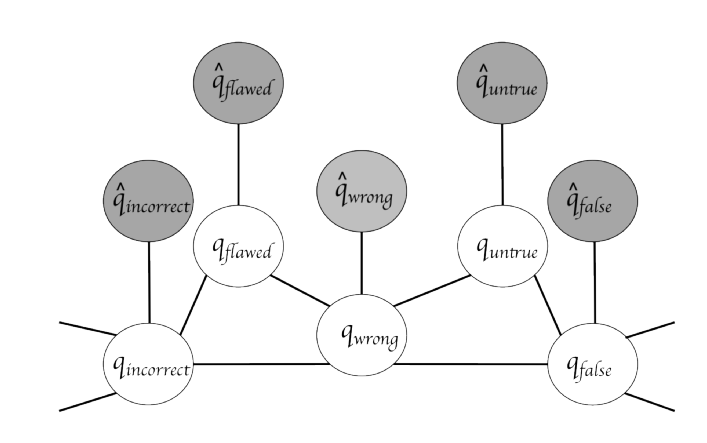
\includegraphics[width=0.85\hsize]{file/retrofit.png}
      
    \column{0.55\hsize}
      \pause
      \begin{enumerate}
       \item 传统工具(word2vec)生成初始向量空间$\hat{Q}$
       \item 根据语义字典生成$\Omega$
       \item 最优(小)化 $\Psi(Q)=$\\  
      \vspace{3mm}
      \end{enumerate}
       \small $\sum_{i=1}^n\biggl[\alpha_i\big\|q_i-\hat{q_i}\big\|^2+\sum_{(i,j)\in E}\beta_{ij}\big\|q_i-q_j\big\|^2\biggl]$

       \pause
	  \begin{columns}[c]
	  \column{0.1\hsize}
	  \column{0.8\hsize}
       \begin{block}{}
	  \begin{itemize}
	   \item (?)$\Psi(Q)$是凸函数$\Rightarrow$沿切线更新$\Rightarrow$ $q_i=\frac{\sum_{j:(i,j)\in E}\beta_{ij}q_j+\alpha_i\hat{q_i}}{\sum_{j:(i,j)\in E}\beta_{ij}+\alpha_i}$
	   \pause
	   \item 10次迭代收敛((?)邻接矩阵距离小于$10^{-2}$)
	  \end{itemize}
       \end{block}
	  \column{0.1\hsize}
	  
	  \end{columns}
	  

  \end{columns}

    

}

\frame{
  \frametitle{Experiment}
  \begin{columns}[c]
   \column{0.65\hsize}
  \centering 顺序模型(Retrofitting with Semantic Lexicons)\\
  \vspace{1mm}
  \centering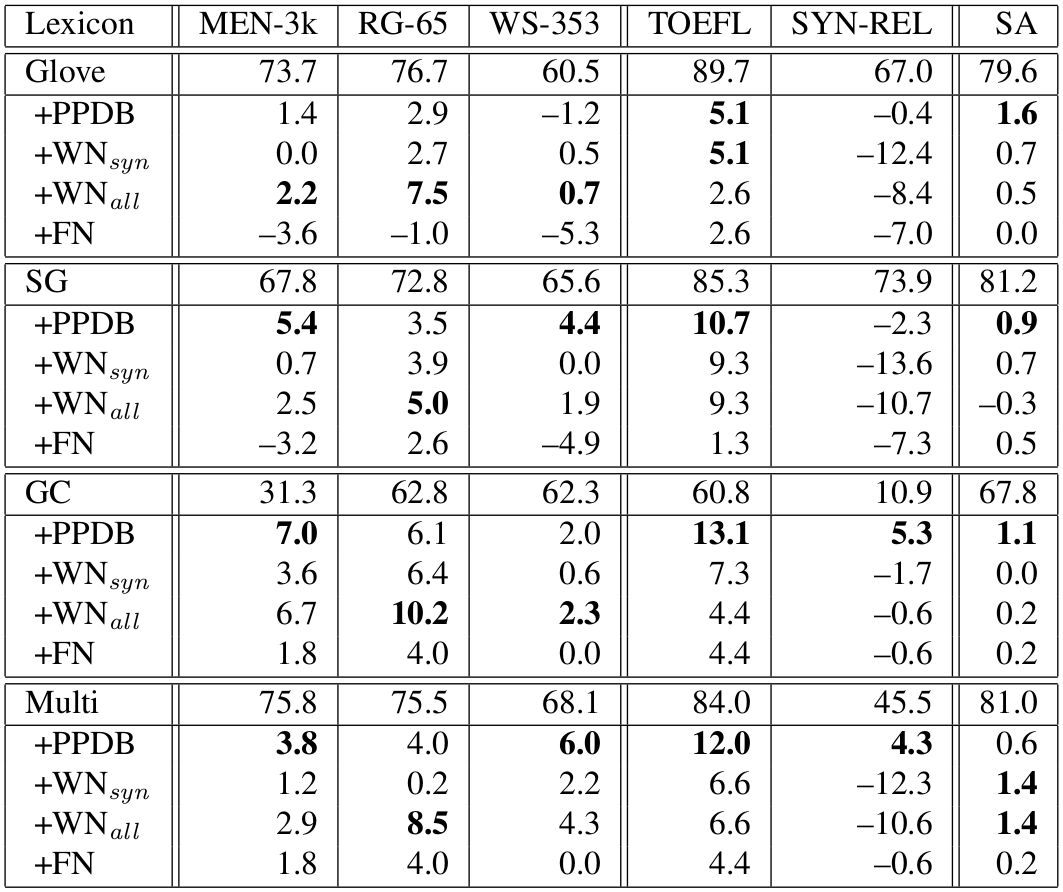
\includegraphics[width=0.95\hsize]{file/experiment_retrofit.png}
  
   \column{0.35\hsize}
      \begin{itemize}
       \item frameNet数据少,效果差
       \item $^{[Append:A]}$语义:Glove好,句法:word2vec好
       \item $PPDB,WN_{all}$好
       \item retrofitting对于句法信息没有提升效果
      \end{itemize}

  \end{columns}

}


\frame{
  \frametitle{联合模型:Semantic Lexicons during Learning}
  修改传统模型的训练过程,加入语义信息
    \begin{block}{\red{lazy} mode}
     核心思想:在传统模型的目标函数中加入体现语义信息的正则项
	\begin{columns}[c]
	    \column{0.1\hsize}
	    \column{0.8\hsize}
	    Q的先验: $p(Q)\propto\exp\Big(-\gamma\sum_{i=1}^n\sum_{j:(i,j)\in E}\beta_{ij}\big\|q_i-q_j\big\|^2\Big)$
	    \column{0.1\hsize}
	\end{columns}
    \begin{enumerate}
     \item $p(Q)$加入目标函数中
     \item 每次更新k个单词的向量(lazy update)
    \end{enumerate}

    \end{block}
    
    \begin{block}{\red{periodic} mode}
     核心思想:递归的过程中每更新k个词后使用下式更新所有的单词向量
     \centering  $q_i=\frac{\sum_{j:(i,j)\in E}\beta_{ij}q_j+\alpha_i\hat{q_i}}{\sum_{j:(i,j)\in E}\beta_{ij}+\alpha_i}$
    \end{block}


}

\frame{
  \frametitle{Experiment}
  联合模型效果测试
  \begin{itemize}
   \item log-bilinear (LBL) vectors为基准(Mnih and Teh, 2012)
   \item \red{lazy} Mode: k=100,000
  \end{itemize}

  \vspace{1mm}
  \centering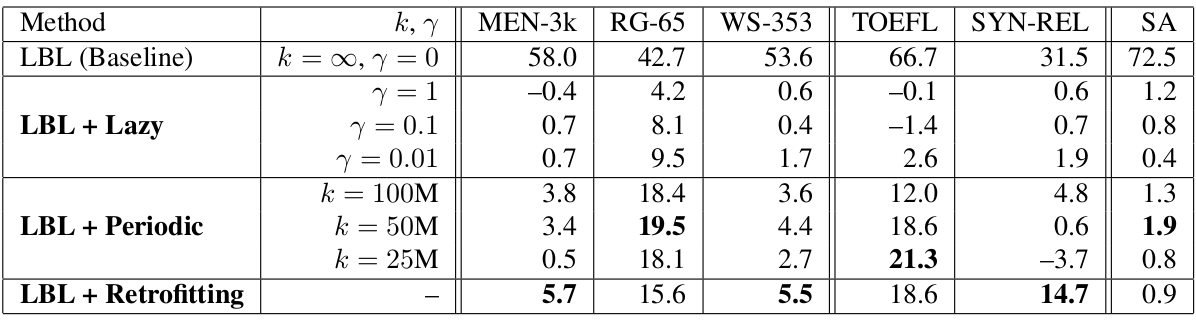
\includegraphics[width=0.95\hsize]{file/experiment_with_train.png}
}

\frame{
  \frametitle{Experiment}
  对比实验
  \begin{block}{Yu and Dredze (2014)}
      \begin{itemize}
       \item word2vec(CBOW)+retrofitting(PPDB)
      \end{itemize}
  \vspace{1mm}
  \centering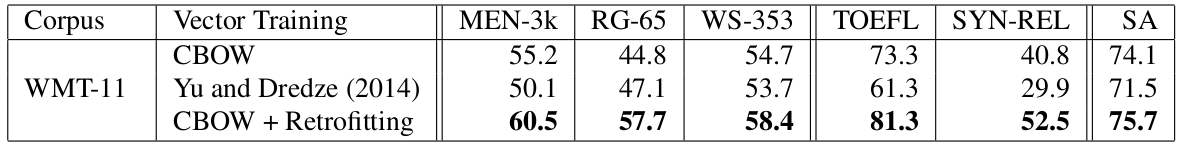
\includegraphics[width=0.95\hsize]{file/experiment_with_WMT.png}
  \end{block}

  \vspace{1mm}
  \begin{block}{Xu et al. (2014)}
      \begin{itemize}
       \item word2vec(CBOW)+retrofitting(PPDB)
      \end{itemize}
  \vspace{1mm}
  \centering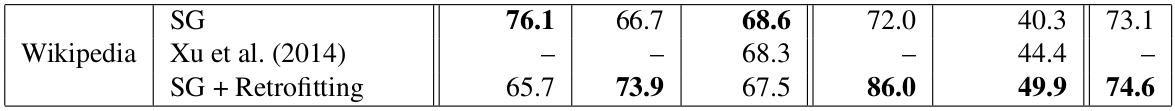
\includegraphics[width=0.95\hsize]{file/experiment_with_wiki.png}
  \end{block}

}

\frame{
  \frametitle{Experiment}
      \begin{columns}[c]
       \column{0.4\hsize}
  多语言效果实验(每种语言独立测试)\\
      \begin{itemize}
       \item retrofitting($WN_{all}$)
      \end{itemize}
  \vspace{1mm}
  \centering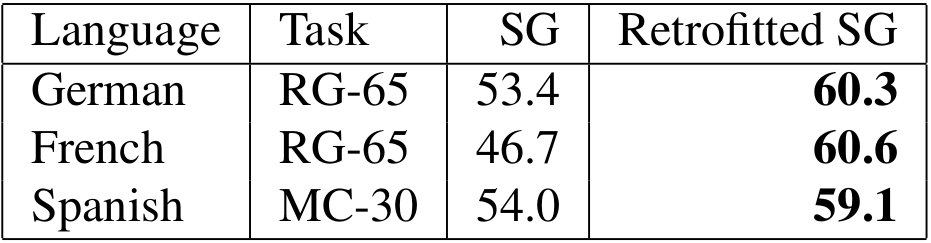
\includegraphics[width=0.95\hsize]{file/experiment_with_multiling.png}
      \pause
       
       \column{0.5\hsize}
   retrofitting和向量长度效用实验\\
  \vspace{1mm}
       \centering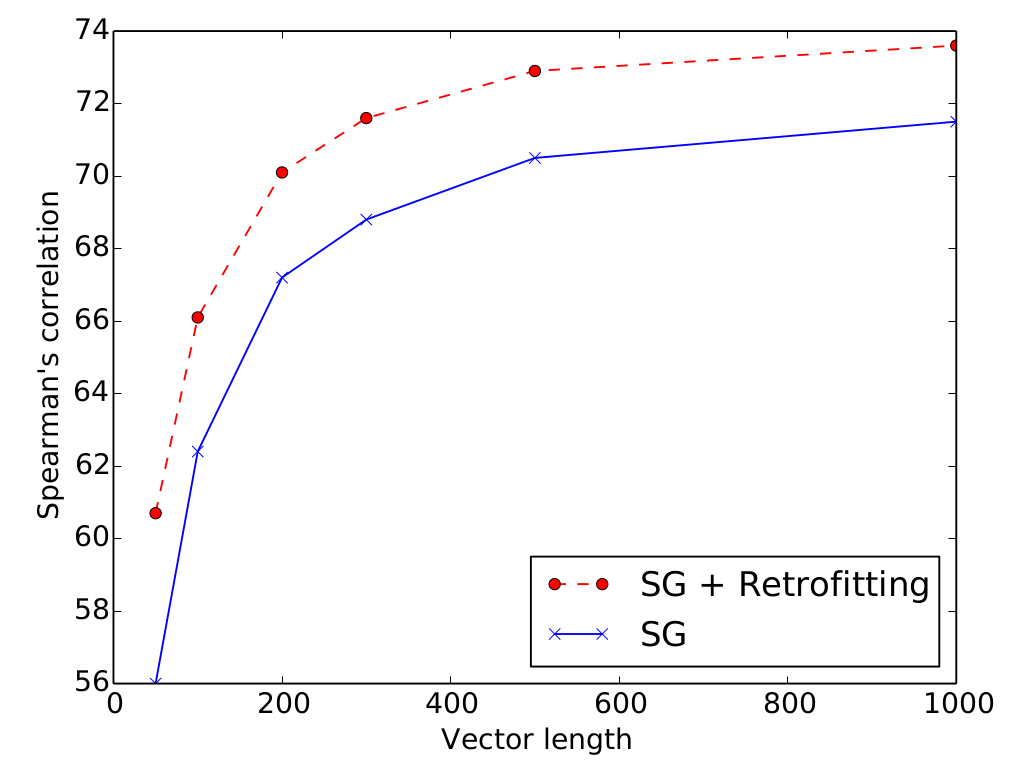
\includegraphics[width=0.75\hsize]{file/experiment_with_vl.png}
       
      \end{columns}


}

\frame{
  \frametitle{Experiment}
  可视化\\
  利用PCA从SG训练得到的100维向量压缩为2维。左右图分别为使用retrofitting前后的向量位置\\
  \vspace{1mm}
       \centering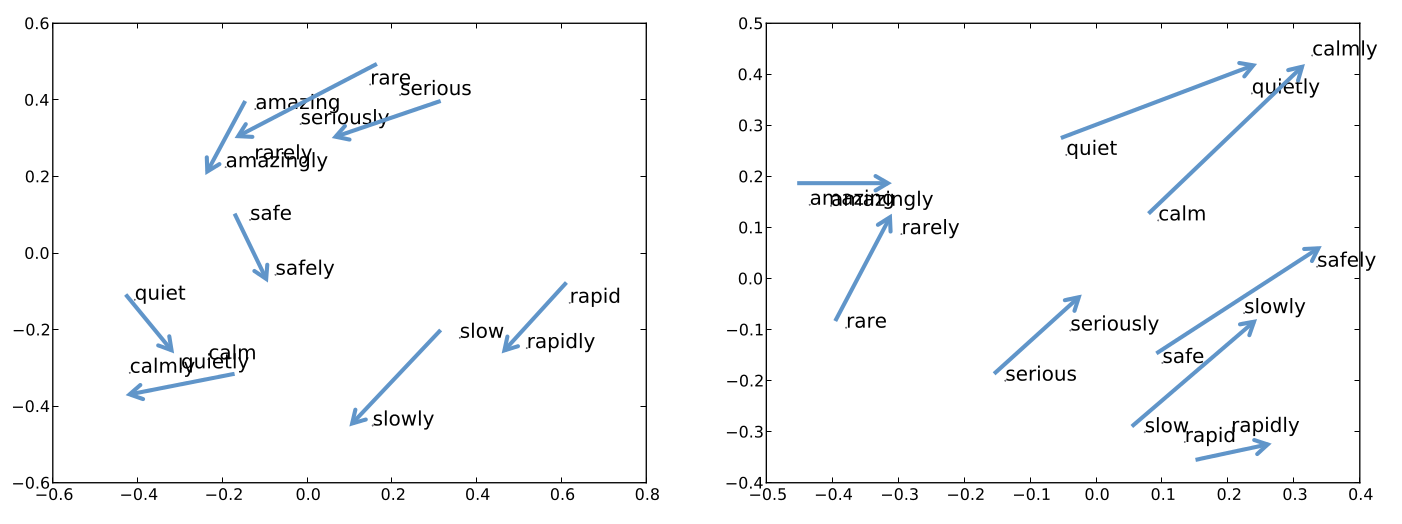
\includegraphics[width=0.75\hsize]{file/experiment_with_visual.png}
  
}

\frame{
  \vspace{30mm}

  \begin{center}
   \Large 谢谢
  \end{center}
  
  \vspace{30mm}
  \tiny 大多数数据集可以在上面找到:http://www.cs.cmu.edu/~mfaruqui/suite.html
}

\frame{
  \frametitle{Append:A}
  GloVe vs word2vec
  \vspace{3mm}
  
\resizebox{6cm}{!}{
\begin{tabular}{|l|l|l|l|}
\hhline{*{4}{-}}
Model & Semantic & Syntactic & Total  \tabularnewline \hhline{*{4}{-}}
GloVe (W+C) & 79.6 & 61.0 & 69.4  \tabularnewline \hhline{*{4}{-}}
word2vec (W) & 72.7 & 65.8 & 68.9  \tabularnewline \hhline{*{4}{-}}
\end{tabular}
}

  \vspace{50mm}
  \tiny https://docs.google.com/document/d/1ydIujJ7ETSZ688RGfU5IMJJsbxAi-kRl8czSwpti15s/mobilebasic
}
\end{document}